\section{Controlling the DC motor from Scilab}
\label{sec:dcm-sci}
\subsection{Controlling the DC motor}
In this section, we discuss how to carry out the experiments of the
previous section from Scilab. We will list the same three experiments,
in the same order.  As mentioned earlier, the shield must be removed from 
the \arduino\ and the \arduino\ needs to be connected to the computer 
with a USB cable, as shown in \figref{arduino}. The reader should go through the instructions given in
\secref{sec:sci-start} before getting started. 

\paragraph{Note:} The readers are advised to affix a small 
(very lightweight) piece of paper at the tip of the shaft of the DC motor. 
That will help them observe the direction of rotation 
of the DC motor while running the experiments. 

\begin{enumerate}
  \item In the first experiment, we will learn how to drive the DC motor
        from Scilab. The code for this experiment is 
        given in  \sciref{sci:dcmotor-clock}. As explained earlier in \secref{sec:light-sci}, 
        we begin with serial port initialization. 
        Next, the code has a command of the following form: 
        \begin{lstlisting}[style=nonumbers]
              cmd_dcmotor_setup(1, H-Bridge type, Motor number, PWM pin 1, PWM pin 2)
        \end{lstlisting}
        As mentioned earlier, this chapter makes use of an H-Bridge circuit which 
        allows direction of the current passing through the DC motor to be changed.
        We are using L293D as an H-Bridge circuit in this book. Thus, we will pass the value 3 for
        H-Bridge type. The Scilab-Arduino toolbox, as explained in \secref{sec:sci-ard-toolbox}, 
        supports three types of H-Bridge circuit. \tabref{table:convention}
        provides the values to be passed for different H-Bridge circuits. 
        Next argument in the command given above is Motor number. Here, we pass the value 1. 
        Finally, we provide the PWM pins to which the DC motor is connected. As 
        shown in \figref{fig:dcmotorconn}, pins 9 and 10 are connected to the
        input of the breakout board. As a result, the command {\tt cmd\_dcmotor\_setup} becomes
        \lstinputlisting[firstline=2,lastline=2]
        {\LocDCMscicode/dcmotor-clock.sce}
        
        \begin{table}
          \centering
          \caption{Values in the \scilab\ command for different H-Bridge circuits}
          \label{table:convention}
          \begin{tabular}{llc}\hline
            Type of H-Bridge circuit & Value \\ \hline
            MotorShield Rev3         & 1                             \\ \hline 
            PMODHB5/L298             & 2                             \\ \hline 
            L293D                    & 3                             \\ \hline
          \end{tabular}
        \end{table}
        
        The next line of \sciref{sci:dcmotor-clock} is of the following form: 
        \begin{lstlisting}[style=nonumbers]
          cmd_dcmotor_run(1, Motor number, [sign] PWM value)
        \end{lstlisting}
        Here, we will pass the value 1 in Motor number.  As mentioned earlier, 
        for each of the PWM pins on \arduino\ board, the input can come from 8 bits.
        Thus, these pins can supply values between $- 255$ and $+ 255$. Positive values correspond to clockwise
        rotation while negative values correspond to anti-clockwise rotation. Based on the PWM value and polarity, 
        corresponding analog voltage is generated.  
        We put a PWM value of 100 to make the DC motor run at an intermediate speed.  
        As a result, the command {\tt cmd\_dcmotor\_run} becomes
        \lstinputlisting[firstline=3,lastline=3]
        {\LocDCMscicode/dcmotor-clock.sce}
        
        The above-mentioned command does not say for how long the motor should run.  This is taken care of
        by the {\tt sleep} command, as given below:
        \lstinputlisting[firstline=4,lastline=4]{\LocDCMscicode/dcmotor-clock.sce}
        With this, the DC motor will run for 3000 milliseconds or 3 seconds. At last, 
        we release the DC motor, as shown below:
        \lstinputlisting[firstline=5,lastline=5]{\LocDCMscicode/dcmotor-clock.sce}
        With the execution of this command, the PWM functionality on the \arduino\ pins
        is ceased.  This has the motor number as an input
        parameter. At last, we close the serial port. 
        
        
        \paragraph{Note:} If the sleep command (at line 4 of \sciref{sci:dcmotor-clock}) 
        were not present, the DC motor will not even run: soon after putting the value 100, 
        the DC motor would be released, leaving no time in between.  On the other hand, if
        the DC motor is not released (\ie\ line number 5 of \sciref{sci:dcmotor-clock} being commented), 
        the DC motor will go on rotating. That's why, it may be inferred that 
        line number 5 of \sciref{sci:dcmotor-clock} is mandatory
        for every program. We encourage the readers to run  \sciref{sci:dcmotor-clock} by commenting
        any one or two of the lines numbered 4, 5 or 6.  Go ahead and do it - you will not break
        anything.  At the most, you may have to unplug the USB cable connected to \arduino\ and
        restart the whole thing from the beginning.
        
  \item It is easy to make the DC motor run in the reverse direction by
        changing the sign of PWM value being written.  This is done in
        \sciref{sci:dcmotor-both}.  In this code, we make the DC motor
        run in one direction for 3 seconds and then make it rotate in the
        reverse direction for 2 seconds.  The rotation in reverse direction
        is achieved by putting $- 100$ in the command {\tt cmd\_dcmotor\_run}, 
        as shown below:
        \lstinputlisting[firstline=5,lastline=5]
        {\LocDCMscicode/dcmotor-both.sce}
        % This makes the green LED light up as well, recall the discussion in \secref{sec:led-pril}.  After
        After adding a {\tt sleep} of 2 seconds, we release the motor by issuing
        the command {\tt cmd\_dcmotor\_release}, followed by closing the serial port:
        \lstinputlisting[firstline=7,lastline=8]
        {\LocDCMscicode/dcmotor-both.sce}
        With this, the motor comes to a halt.  
        % This turns the green LED off as well.
        
  \item Next, we make the DC motor run in forward and reverse
        directions, in a loop.  This is done through
        \sciref{sci:dcmotor-loop}.  We first write PWM $+100$ for 3
        seconds.  After that, halt the motor for 2 seconds by writing zero PWM value.  
        Next, make the motor rotate in the reverse direction by writing PWM $-100$ for two seconds.  
        Next, we make the motor stop for one second. This procedure is put in a {\tt for} loop which runs for 4 iterations.
        At last, we release the motor by issuing the command {\tt cmd\_dcmotor\_release}, followed by closing the serial port
        
\end{enumerate}

% \subsection{Initialization}
% In all the experiments in this section, we need to initialize the DC
% motor first, using a \scilab\ command of the following type:

% \begin{lstlisting}[style=nonumbers]
%   cmd_dcmotor_setup(1,H-Bridge type,Motor number,PWM pin 1,PWM pin 2)
% \end{lstlisting}
% As mentioned earlier, number 1 in the above list refers to the
% \arduino\ board.  We now discuss how to choose values for the other
% parameters in this command.  As mentioned above, there are many
% H-bridge IC manufacturers.  The inbuilt function {\tt
%     cmd\_dcmotor\_setup} can work with most of the widely used ICs,
% through a suitable input parameter.  Users have to provide the type
% number of the breakout board they have.  Popular numbering convention
% for different types of DC motor breakout boards is given in
% \tabref{table:convention}.  For example, L293D is type 3.  Next, we
% have to provide the motor number we want to control.  In our case, it
% is number 1.  Finally we want to provide PWM pin numbers on \arduino.
% As mentioned earlier, we are using pins 10 and 11.  In
% \tabref{tab:dcmotor-init}, we list the choices that we have made.
% Inserting these parameter values in the above shown \scilab\ command,
% we get the following command \\
% \lstinputlisting[firstline=2,lastline=2]
% {\LocDCMscicode/dcmotor-clock.sce}
% which is line number 2 in \sciref{sci:dcmotor-clock}.  We have already
% seen 
% the first two lines of this code and hence will not explain here.  We
% will add more lines to this code as we go along.




% % \begin{table}
% %   \centering
% %   \caption{Parameters for DC motor initialization}
% %   \label{tab:dcmotor-init}
% %   \begin{tabular}{|l|c|} \hline
% %     Parameter     & Value \\ \hline
% %     H-Bridge type & 3     \\ 
% %     Motor number  & 1     \\
% %     PWM 1 pin     & 9     \\
% %     PWM 2 pin     & 10    \\ \hline
% %   \end{tabular}
% % \end{table}

% \subsection{Rotation for a specified time}
% \label{sec:dc-both}
% We will now explain how to run the DC motor.  We have to provide motor
% number and the PWM value.  The \scilab\ command is of the form,
% \begin{lstlisting}[style=nonumbers]
%   cmd_dcmotor_run(1,Motor number,(sign)(PWM value))
% \end{lstlisting}
% Motor number is 1, as mentioned earlier.  Considering that the input
% to a PWM pin comes from two 8 digital pins, we can provide values
% between $-255$ and +255. Positive values correspond to clockwise
% rotation while negative values correspond to anti-clockwise rotation.
% Based on the PWM value and polarity, corresponding analog voltage is
% generated.  We put a PWM value of 100 to make the DC motor to
% run at an intermediate speed.  Assigning these values, we get the
% following command:
% \lstinputlisting[firstline=3,lastline=3]{\LocDCMscicode/dcmotor-clock.sce}
% This is line number 3 in \sciref{sci:dcmotor-clock}.  This command
% does not say for how long the motor should run.  This is taken care of
% by the {\tt sleep} statement.  The units of sleep are milliseconds.
% For example, line number 4 of \sciref{sci:dcmotor-clock}, given next,
% says that \scilab\ should go to sleep for three seconds.
% \lstinputlisting[firstline=4,lastline=4]{\LocDCMscicode/dcmotor-clock.sce}

% Line number 5 of \sciref{sci:dcmotor-clock}, shown below, is mandatory
% for every program.
% \lstinputlisting[firstline=5,lastline=5]{\LocDCMscicode/dcmotor-clock.sce}
% It releases the DC motor.  The PWM functionality on the \arduino\ pins
% is ceased using this command.  This has the motor number as an input
% parameter.

% If the sleep command discussed above were not present, the DC motor
% will not even run: soon after putting the value 100, the DC motor
% would be released, leaving no time in between.  If on the other hand,
% the DC motor is not released (\ie\ line number 6 being absent), the DC
% motor will go on rotating.  Line number 6 of \sciref{sci:dcmotor-clock}
% closes the serial port.

% We encourage you to run the above code without either line numbers 4,
% 5 or 6 or all combinations.  Go ahead and do it - you will not break
% anything.  At the most, you may have to unplug the USB cable and
% restart the whole thing from the beginning.

% \sciref{sci:dcmotor-clock} can easily be extended to make the DC motor
% run in both directions.  The modified code is available in
% \sciref{sci:dcmotor-both}.

\begin{exercise}
  Carry out the following exercise:
  \begin{enumerate}
    \item Try out some of the suggestions given above, \ie\ removing
          certain numbers from the code. 
    \item See if the DC motor runs if you put 1 instead of 100 as the PWM
          value.  Explain why it does not run.  Find out the smallest value at
          which it will start running.
  \end{enumerate}
\end{exercise}

% \subsection{Using the capabilities of \scilab}
% Given that Scilab has a powerful programming syntax, a lot of
% different experiments can be tried out.  We illustrate a few in this
% section.  We begin with a {\tt for loop}.

% In the previous section, we presented \sciref{sci:dcmotor-both}, where
% we made the motor run in both directions, five seconds in the
% clockwise direction and two seconds in reverse.  This code can be
% embedded in a loop and the motor be made to repeat a certain number of
% times.  This idea is implemented through \sciref{sci:dcmotor-loop}.
% Through the {\tt for loop} in between line numbers 3 and 8, we make
% the DC motor repeat four times the cycle containing one rotation in
% each direction. 
%  \figref{fig:dcmotorfc} explains the entire operation
% through a flowchart.
% \begin{figure}
% \centering
% 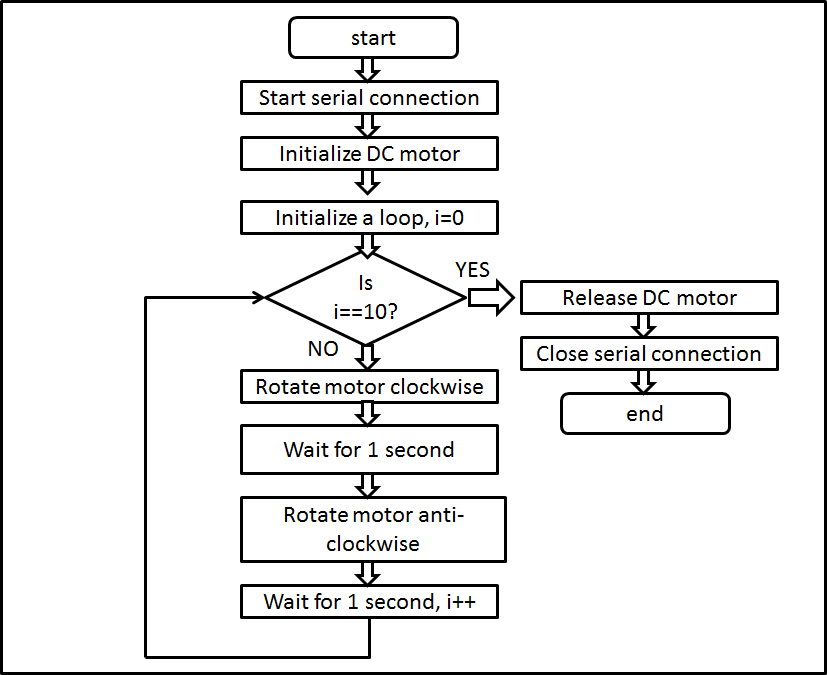
\includegraphics[width=\lgfig]{\LocDCMfig/dcmotorflowchart.png}
% \caption{Flowchart}
% \label{fig:dcmotorfc}
% \end{figure}

% It is not difficult to see how some of the other features of the
% \scilab\ programming language can be used along with this DC motor.
% For example, it is possible to read a temperature value and based on
% its value, start or stop the motor.  For real world applications, one
% has to provide extra current carrying capabilities through external
% hardware.  

\subsection{Scilab Code}
\label{sec:dcmotor-scilab-code}
\addtocontents{cod}{\protect\addvspace{\codclr}}

\begin{scicode}
  \ccaption{Rotating the DC motor}
  {Rotating the DC motor.  Available at
    \LocDCMscibrief{dcmotor-clock.sce}.}
  \label{sci:dcmotor-clock}
  \lstinputlisting{\LocDCMscicode/dcmotor-clock.sce}
\end{scicode}

\begin{scicode}
  \ccaption{Rotating the DC motor in both directions}
  {Rotating DC motor in both directions.  Available at
    \LocDCMscibrief{dcmotor-both.sce}.}
  \label{sci:dcmotor-both}
  \lstinputlisting{\LocDCMscicode/dcmotor-both.sce}
\end{scicode}

\begin{scicode}
  \ccaption{Rotating the DC motor in both directions in a loop}{Rotating
    the DC motor in both directions in a loop.
    Available at
    \LocDCMscibrief{dcmotor-loop.sce}.}
  \label{sci:dcmotor-loop}
  \lstinputlisting{\LocDCMscicode/dcmotor-loop.sce}
\end{scicode}

\section{Controlling the DC motor from Xcos}
In this section, we will see how to drive the DC motor from Scilab Xcos. 
We will carry out the same three experiments as in the previous
sections. For each experiment, we will give the location of the zcos file and the
parameters to set.  The reader should go through the instructions
given in \secref{sec:xcos-start} before getting started.  


% If the
% rotation of the DC motor is blocked by any obstacle in any of the
% experiments given below, you may want to hold it in your hand and let
% it run unhindered.

\begin{enumerate}
  \item First we will see a simple code that drives the DC motor for a
        specified time.  When the file required for this experiment is
        invoked, one gets the GUI as in \figref{fig:dcmotor-clock}.  In
        the caption of this figure, one can see where to locate the file.
        
        \begin{figure}
          \centering
          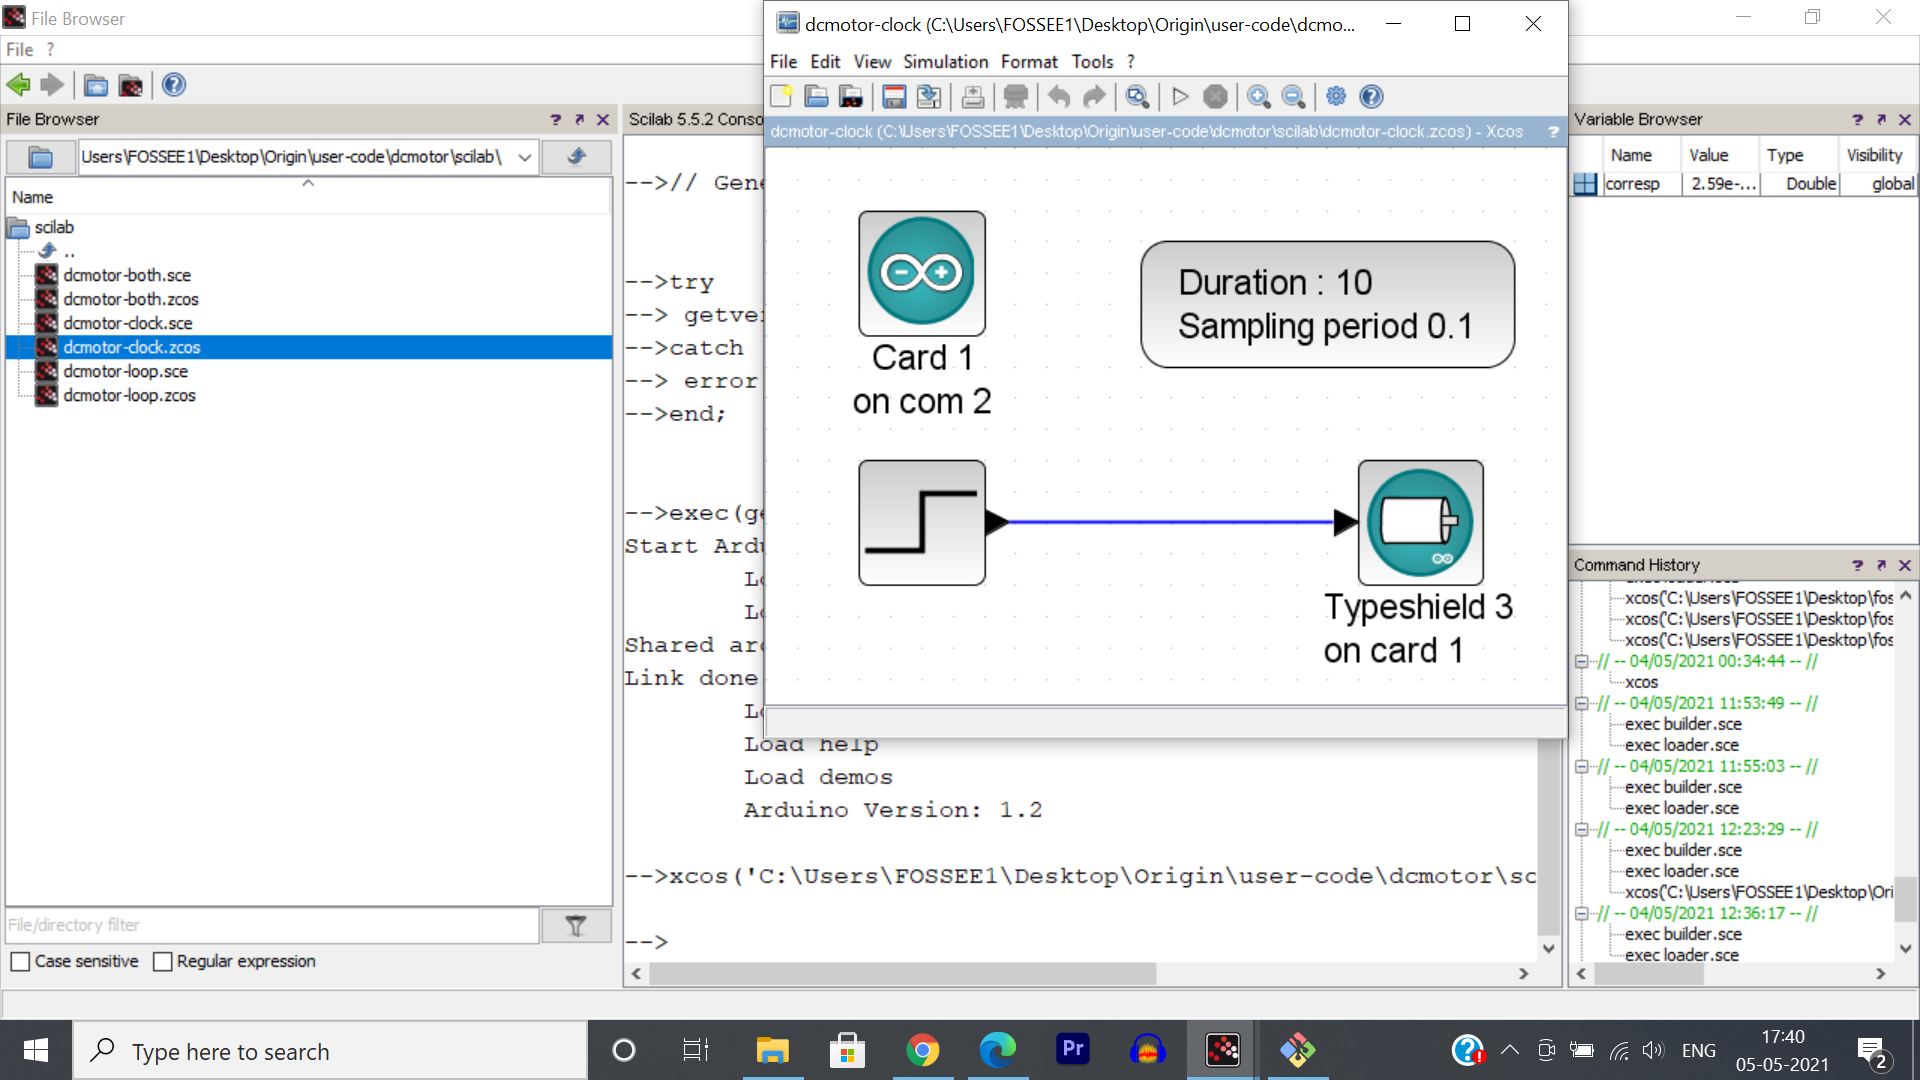
\includegraphics[width=\smfig]{\LocDCMfig/dcmotor-clock.png}
          \caption[Control of DC motor for a specified time from Xcos]
          {Control of DC motor for a specified time from Xcos.  This is what
            one sees when \LocDCMscibrief{dcmotor-clock.zcos}, is
            invoked.}
          \label{fig:dcmotor-clock}
        \end{figure}
        
        We will next explain how to set the parameters for this simulation.
        To set value on any block, one needs to right click and open the
          {\tt Block Parameters} or double click.  The values for each block
        is tabulated in \tabref{tab:dcmotor-clock}.  In case of {\tt
            DCMOTOR\_SB}, enter 3 to indicate for L293D board.  After clicking
        on OK, another dialog box will pop up.  In that, enter the PWM pin numbers
        as 9 and 10 and click OK.  
        All other parameters are to be left
        unchanged.
        \begin{table}
          \centering
          \caption{Xcos parameters to drive the DC motor for a specified time}
          \label{tab:dcmotor-clock}
          \begin{tabular}{llc} \hline
            Name of the block & Parameter name             & Value     \\ \hline
            ARDUINO\_SETUP    & Identifier of Arduino Card & 1         \\
                              & Serial com port number     & 2\portcmd \\ \hline
            TIME\_SAMPLE      & Duration of acquisition(s) & 10        \\
                              & Sampling period(s)         & 0.1       \\ \hline
            DCMOTOR\_SB       & Type of Shield             & 3         \\
                              & Arduino card number        & 1         \\ 
                              & PWM pin numbers            & 9 10      \\ 
                              & Motor number               & 1         \\ \hline
            STEP\_FUNCTION    & Step time                  & 5         \\
                              & Initial Value              & 100       \\
                              & Final Value                & 0         \\ \hline
          \end{tabular}
        \end{table}
        
        % Can you find out for how long the DC motor will run when this program
        % is executed?  In which block do we provide this information?  The
        % answer is that the DC motor will stop only when we terminate the
        % program.  As in the previous experiments, we can terminate the Xcos
        % program by pressing the stop button.  The DC motor gets released when
        % the stop button is pressed.
        
        
        
  \item Next, we will describe the Xcos code that drives the DC motor in
        both forward and reverse directions.  When the file required for
        this experiment is invoked, one gets the GUI as in
        \figref{fig:dcmotor-both}.  In the caption of this figure, one can
        see where to locate the file.
        
        \begin{figure}
          \centering
          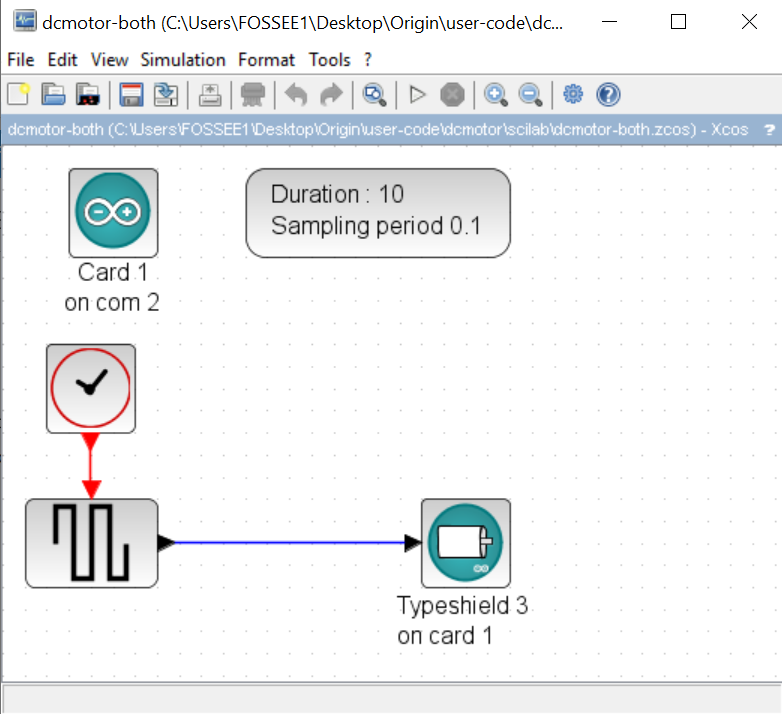
\includegraphics[width=\smfig]{\LocDCMfig/dcmotor-both.png}
          \caption[Xcos control of the DC motor in forward and reverse
            directions]{Xcos control of the DC motor in forward and reverse
            directions.  This is what one sees when
            \LocDCMscibrief{dcmotor-both.zcos}, is invoked.}
          \label{fig:dcmotor-both}
        \end{figure}
        
        We will next explain how to set the parameters for this simulation.
        To set value on any block, one needs to right click and open the
          {\tt Block Parameters} or double click.  The values for each block
        is tabulated in \tabref{tab:dcmotor-both}.  All other parameters are
        to be left unchanged.
        \begin{table}
          \centering
          \caption{Xcos parameters to drive the DC motor in forward and
            reverse directions}
          \label{tab:dcmotor-both}
          \begin{tabular}{llc} \hline
            Name of the block & Parameter name             & Value     \\ \hline
            ARDUINO\_SETUP    & Identifier of Arduino Card & 1         \\
                              & Serial com port number     & 2\portcmd \\ \hline
            TIME\_SAMPLE      & Duration of acquisition(s) & 10        \\
                              & Sampling period(s)         & 0.1       \\ \hline
            DCMOTOR\_SB       & Type of Shield             & 3         \\
                              & Arduino card number        & 1         \\ 
                              & PWM pin numbers            & 9 10      \\ 
                              & Motor number               & 1         \\ \hline
            STEP\_FUNCTION    & Step time                  & 5         \\
                              & Initial Value              & 100       \\
                              & final value                & 0         \\ \hline
            CLOCK\_c          & Period                     & 1         \\
                              & Initialisation Time        & 0.1       \\ \hline
          \end{tabular}
        \end{table}
        
  \item Next, we will describe the Xcos code that drives the DC motor in
        a loop.  When the file required for
        this experiment is invoked, one gets the GUI as in
        \figref{fig:dcmotor-loop}.  In the caption of this figure, one can
        see where to locate the file.
        
        \begin{figure}
          \centering
          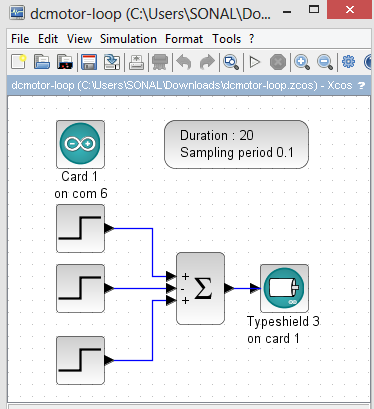
\includegraphics[width=\smfig]{\LocDCMfig/dcmotor-loop.png}
          \caption[Xcos control of the DC motor in both directions in a loop]
          {Xcos control of the DC motor in both directions in a loop.  This is what one sees when
            \LocDCMscibrief{dcmotor-loop.zcos}, is invoked.}
          \label{fig:dcmotor-loop}
        \end{figure}
        
        We will next explain how to set the parameters for this simulation.
        To set value on any block, one needs to right click and open the
          {\tt Block Parameters} or double click.  The values for each block
        is tabulated in \tabref{tab:dcmotor-loop}.  All other parameters are
        to be left unchanged.
        \begin{table}
          \centering
          \caption{Xcos parameters to drive the DC motor in a loop}
          \label{tab:dcmotor-loop}
          \begin{tabular}{llc} \hline
            Name of the block & Parameter name             & Value     \\ \hline
            ARDUINO\_SETUP    & Identifier of Arduino Card & 1         \\
                              & Serial com port number     & 2\portcmd \\ \hline
            TIME\_SAMPLE      & Duration of acquisition(s) & 10        \\
                              & Sampling period(s)         & 0.1       \\ \hline
            DCMOTOR\_SB       & Type of Shield             & 3         \\
                              & Arduino card number        & 1         \\
                              & PWM pin numbers            & 9 10      \\ 
                              & Motor number               & 1         \\ \hline
            STEP\_FUNCTION 1  & Step time                  & 3         \\
                              & Initial Value              & 100       \\
                              & Final Value                & 0         \\ \hline
            STEP\_FUNCTION 2  & Step time                  & 5         \\
                              & Initial Value              & 0         \\
                              & Final Value                & 100       \\ \hline
            STEP\_FUNCTION 3  & Step time                  & 7         \\
                              & Initial Value              & 0         \\
                              & Final Value                & 100       \\ \hline
            BIGSOM\_f         & Inputs ports signs/gain    & [1;-1;1]  \\ \hline
          \end{tabular}
        \end{table}
\end{enumerate}


%\section{Do we need any of these? \redcolor{Manas, please answer}}
%   \begin{figure}
%     \centering
%     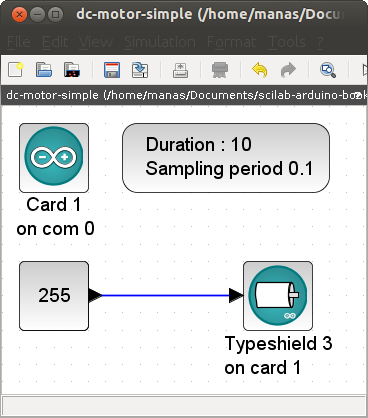
\includegraphics[width=\smfig]{\LocDCMfig/dc-motor-simple.png}
%     \caption[Control of DC motor from Xcos]{Control of DC motor from
%       Xcos.  This is what one sees when {\tt
%         \LocDCMscibrief/dc-motor-simple.zcos} is invoked.}
%     \label{fig:dcm-xcos-simple}
%   \end{figure}



% \begin{enumerate}
% \item Card 1 on com 5 block: Right-click and open the block properties
%   or double click on this block.  In the resulting dialog window,
%   enter the com port number of your system.
% \item Typeshield 1 on card 1: Following the procedure mentioned above,
%   make sure that the entry for this block is 3, which corresponds to
%   L293D breakout board, as explained in \tabref{table:convention}. 
% \end{enumerate}
% Leave the other blocks unchanged.

% This Xcos program is used to put a specific PWM value to the DC motor.
% We can right click (or double click) on any block and see what
% parameter values are present in it.  By doing this, we can see that
% this program is used to put in a PWM value of 255.  Start executing
% the program by pressing the right arrow key.  

\begin{exercise} 
  Carry out the following exercise:
  \begin{enumerate}
    \item Keep reducing the PWM value and find out the minimum value
          required to run the DC motor.  Is this value in agreement with what
          we found in the previous section?
    \item Change the PWM value to $-100$ and check if the DC motor rotates
          in the opposite direction.
    \item Find out the smallest PWM value required to make the motor run
          in the opposite direction.  That is, find the least count for both
          directions.
    \item Come up with a method to rotate the motor in two directions for
          different time periods.
  \end{enumerate}
\end{exercise}

